\chapter{Integration, Implementation and Test Plan}

\section{Overview and Implementation}

This final chapter outlines the system's implementation process, along with the strategies for integration and testing. A Bottom-Up approach will be used as the guiding methodology.

This strategy involves starting from the lower levels of the "uses" hierarchy, beginning with the development of smaller, independent modules that do not depend on other components to function. Each of these modules will be accompanied by a driver specifically created for testing purposes. Once a module has been implemented and verified, it will be integrated into the system, replacing its corresponding driver. However, a new driver will be developed for the next module to ensure continuous testing.

By following this approach, several functional subsystems will be progressively developed and tested before being combined into the final system. The Bottom-Up method supports incremental integration, allowing for early detection of bugs and errors since testing occurs in smaller, manageable segments as each module is completed. Additionally, this strategy enables parallel development, as independent teams can work simultaneously on different system components.

\section{Features Identification}

\begin{enumerate}[label={\textbf{[F\arabic*]}}, leftmargin=1.52cm]
    \item \textbf{Login and Registration Features:} This are the features needed by all of the user of the platform: Students, Companies and Universities. These features play a pivotal role like ensuring proper data validation and secure storage of registration details, managing the verification process for universities, implementing workflows for account recovery and activation, ensuring system security using secure login mechanisms and as such will be the first to be implemented.
    \item \textbf{Creation Feature:} This set of features includes tools for creating and enhancing content, such as filling out questionnaires, submitting applications, and improving CVs.
    \item \textbf{View Features:} This set of features includes all the action of visualization included in the platform such as looking at internships. They need the corresponding \textbf{F3}, \textbf{F4} features in order to work and are essential for other features
    \item \textbf{Search Features:} These features cover all platform operations related to searching for content, such as finding internships or candidates. 
    \item \textbf{Internship Features:} These features provide access to internship related information, such as internship details and progress tracking. These also include joining and applying for an internship as well as replying to the questionnaires in case of acceptance 
    \item \textbf{Evaluation Features:} This category includes the operations of evaluating internship applications and interview performances.
    \item \textbf{Message Features:} These features enable controlled messaging between all platform users.
    \item \textbf{Recommendation Features:} This set involves personalized recommendations for students and companies, suggesting internships for students and suitable candidates for companies.
    \item \textbf{Complaints Features:} These features allow users to submit complaints to the university once an internship has started, facilitating issue resolution.
    \item \textbf{Feedback Features:} This set covers feedback-related actions, including both submitting feedback and responding to feedback requests.
    \item \textbf{Notification Features:} These features handle the delivery of notifications regarding platform events and updates. They will be the last features implemented
    

\end{enumerate}

\section{Overview and Implementation}

Component integration and system testing should begin as soon as the DBMS and host server are prepared. Connections to the Mailing System and External Tools are not immediately required but will be essential once their respective features are incorporated. As previously mentioned, the integration process will follow a bottom-up approach.

We will start our model that will be tested alongside a driver.

\begin{figure}[H]
    \centering
    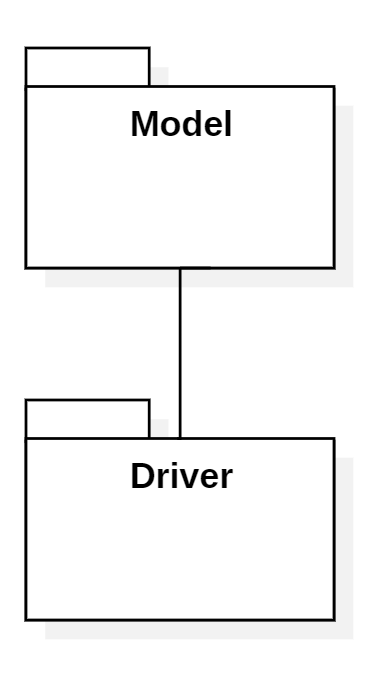
\includegraphics[width=0.2\linewidth]{DD/Images/Implementation Images/basic.png}
    \label{fig:enter-label}
\end{figure}

Once integration begins, the initial features to be implemented will be Log-in and Sign-up.

\begin{figure}[H]
    \centering
    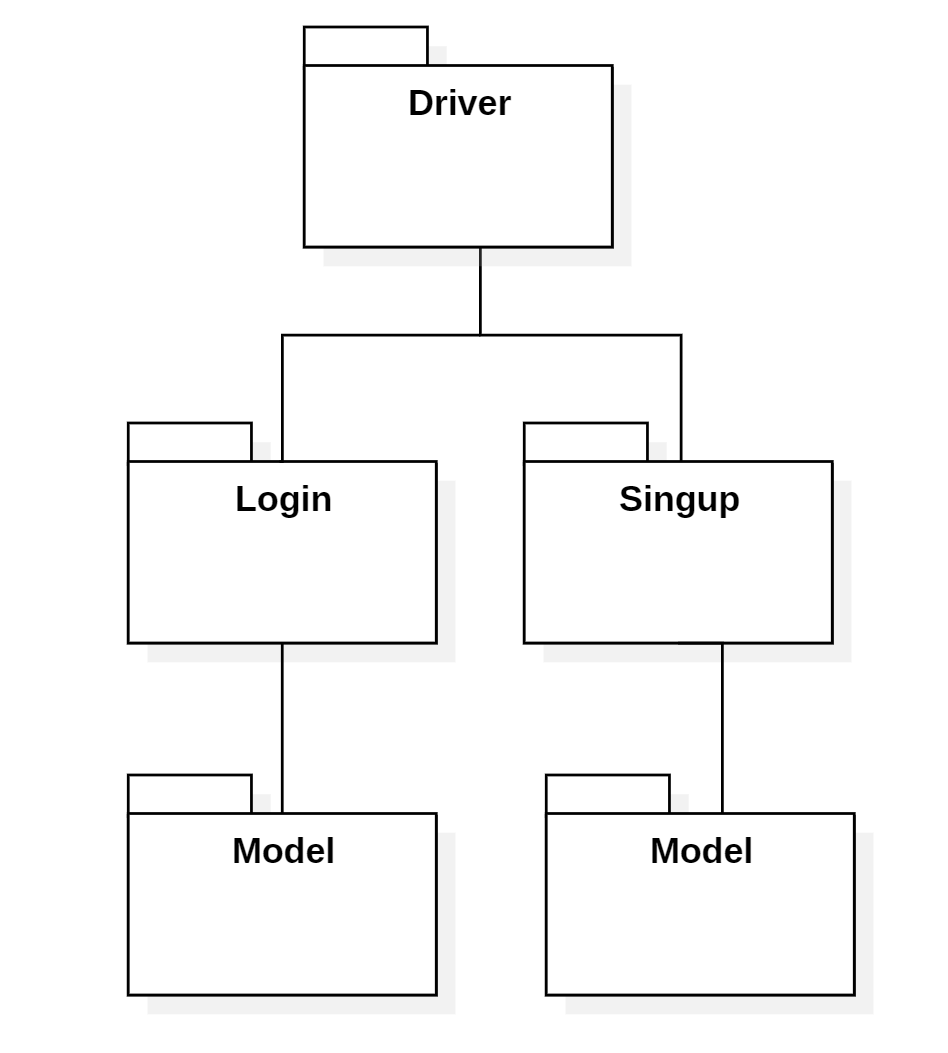
\includegraphics[width=0.45\linewidth]{DD/Images/Implementation Images/loginsingup.png}
    \label{fig:enter-label}
\end{figure}

After testing the Log-in and Sign-up features, the remaining identified features will be added gradually, step by step. 

\begin{figure}[H]
    \centering
    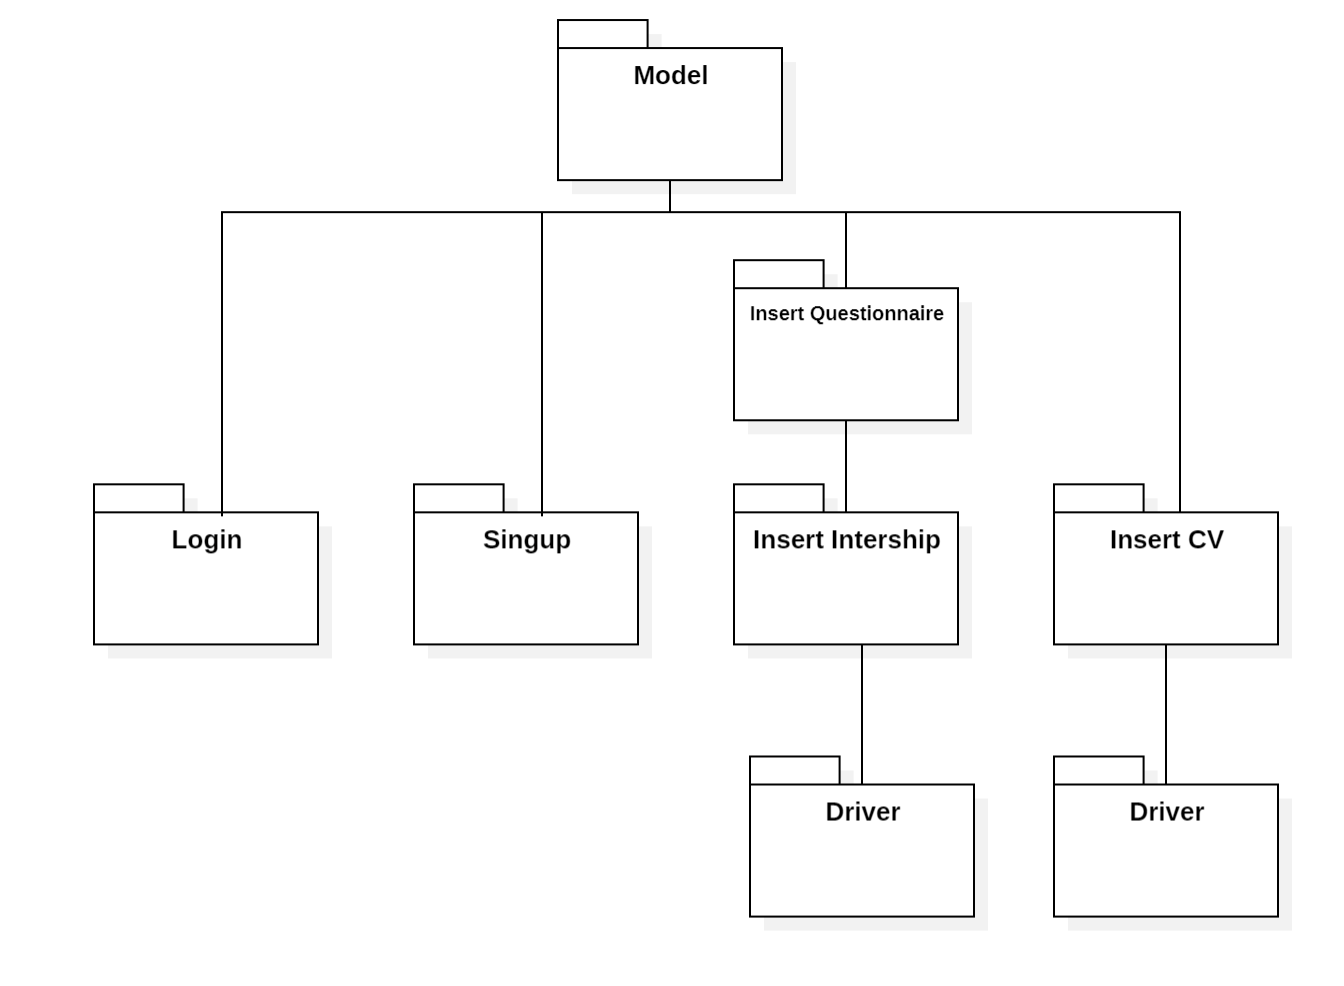
\includegraphics[width=0.75\linewidth]{DD/Images/Implementation Images/insert.png}
    \label{fig:enter-label}
\end{figure}

In the following, additional identified features will progressively be integrated, continuing the step-by-step approach.

\begin{figure}[H]
    \centering
    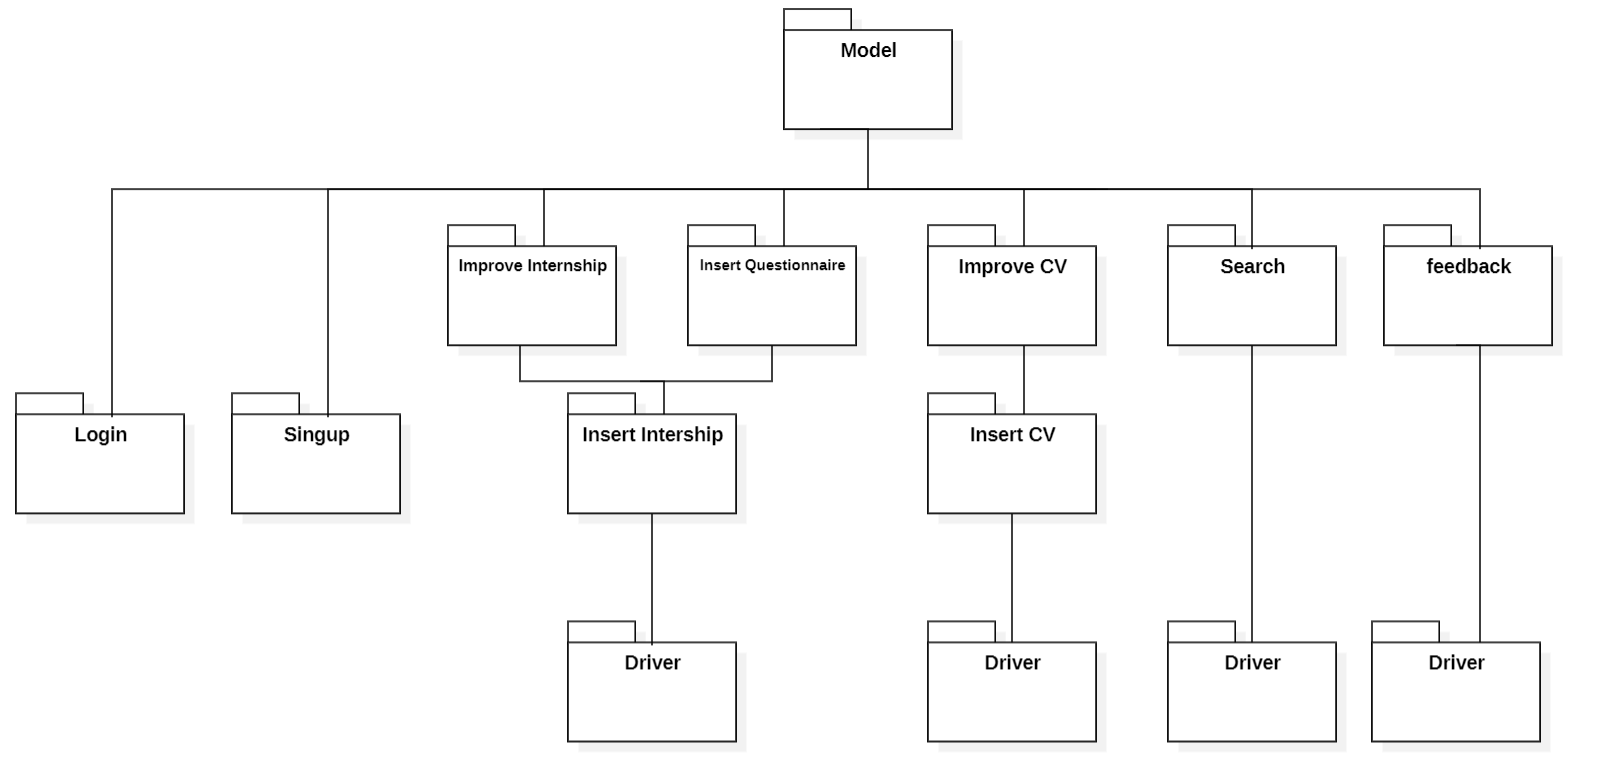
\includegraphics[width=1\linewidth]{DD//Images//Implementation Images/improvement search and feedback.png}
    \label{fig:enter-label}
\end{figure}

Finally, the last set of features will be added, completing the integration process.

\begin{figure}[H]
    \centering
    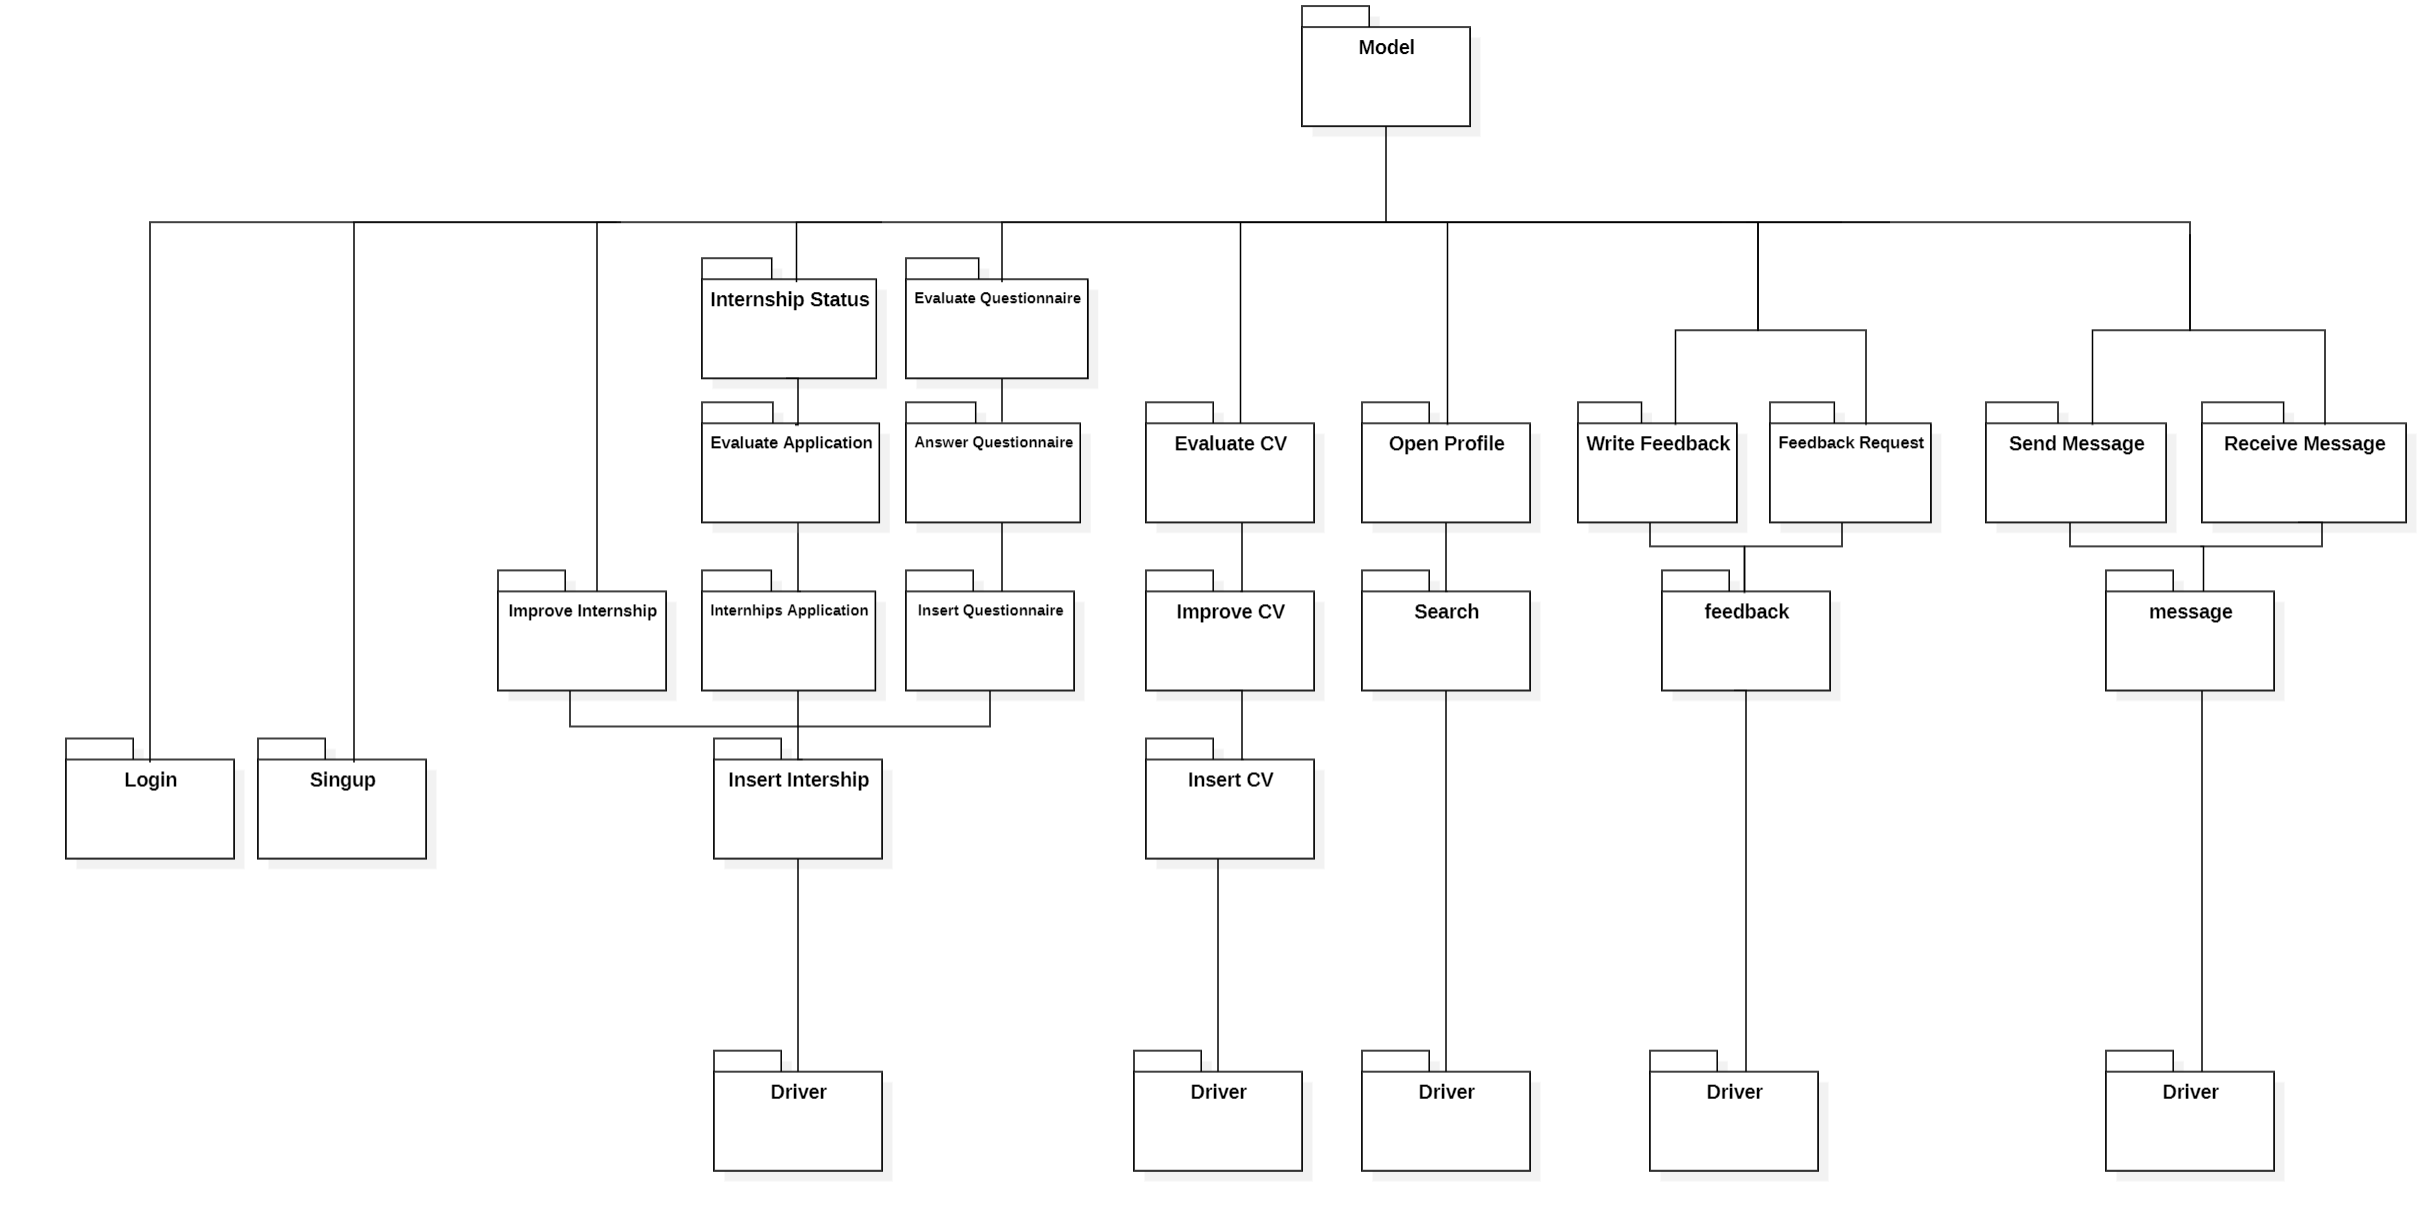
\includegraphics[width=1\linewidth]{DD//Images//Implementation Images/finalwithnomanagers.png}
    \label{fig:enter-label}
\end{figure}

For simplicity, some of the previously integrated components will be consolidated within the Managers component. They will be grouped together to make the system's graph more comprehensible.

\begin{figure}[H]
    \centering
    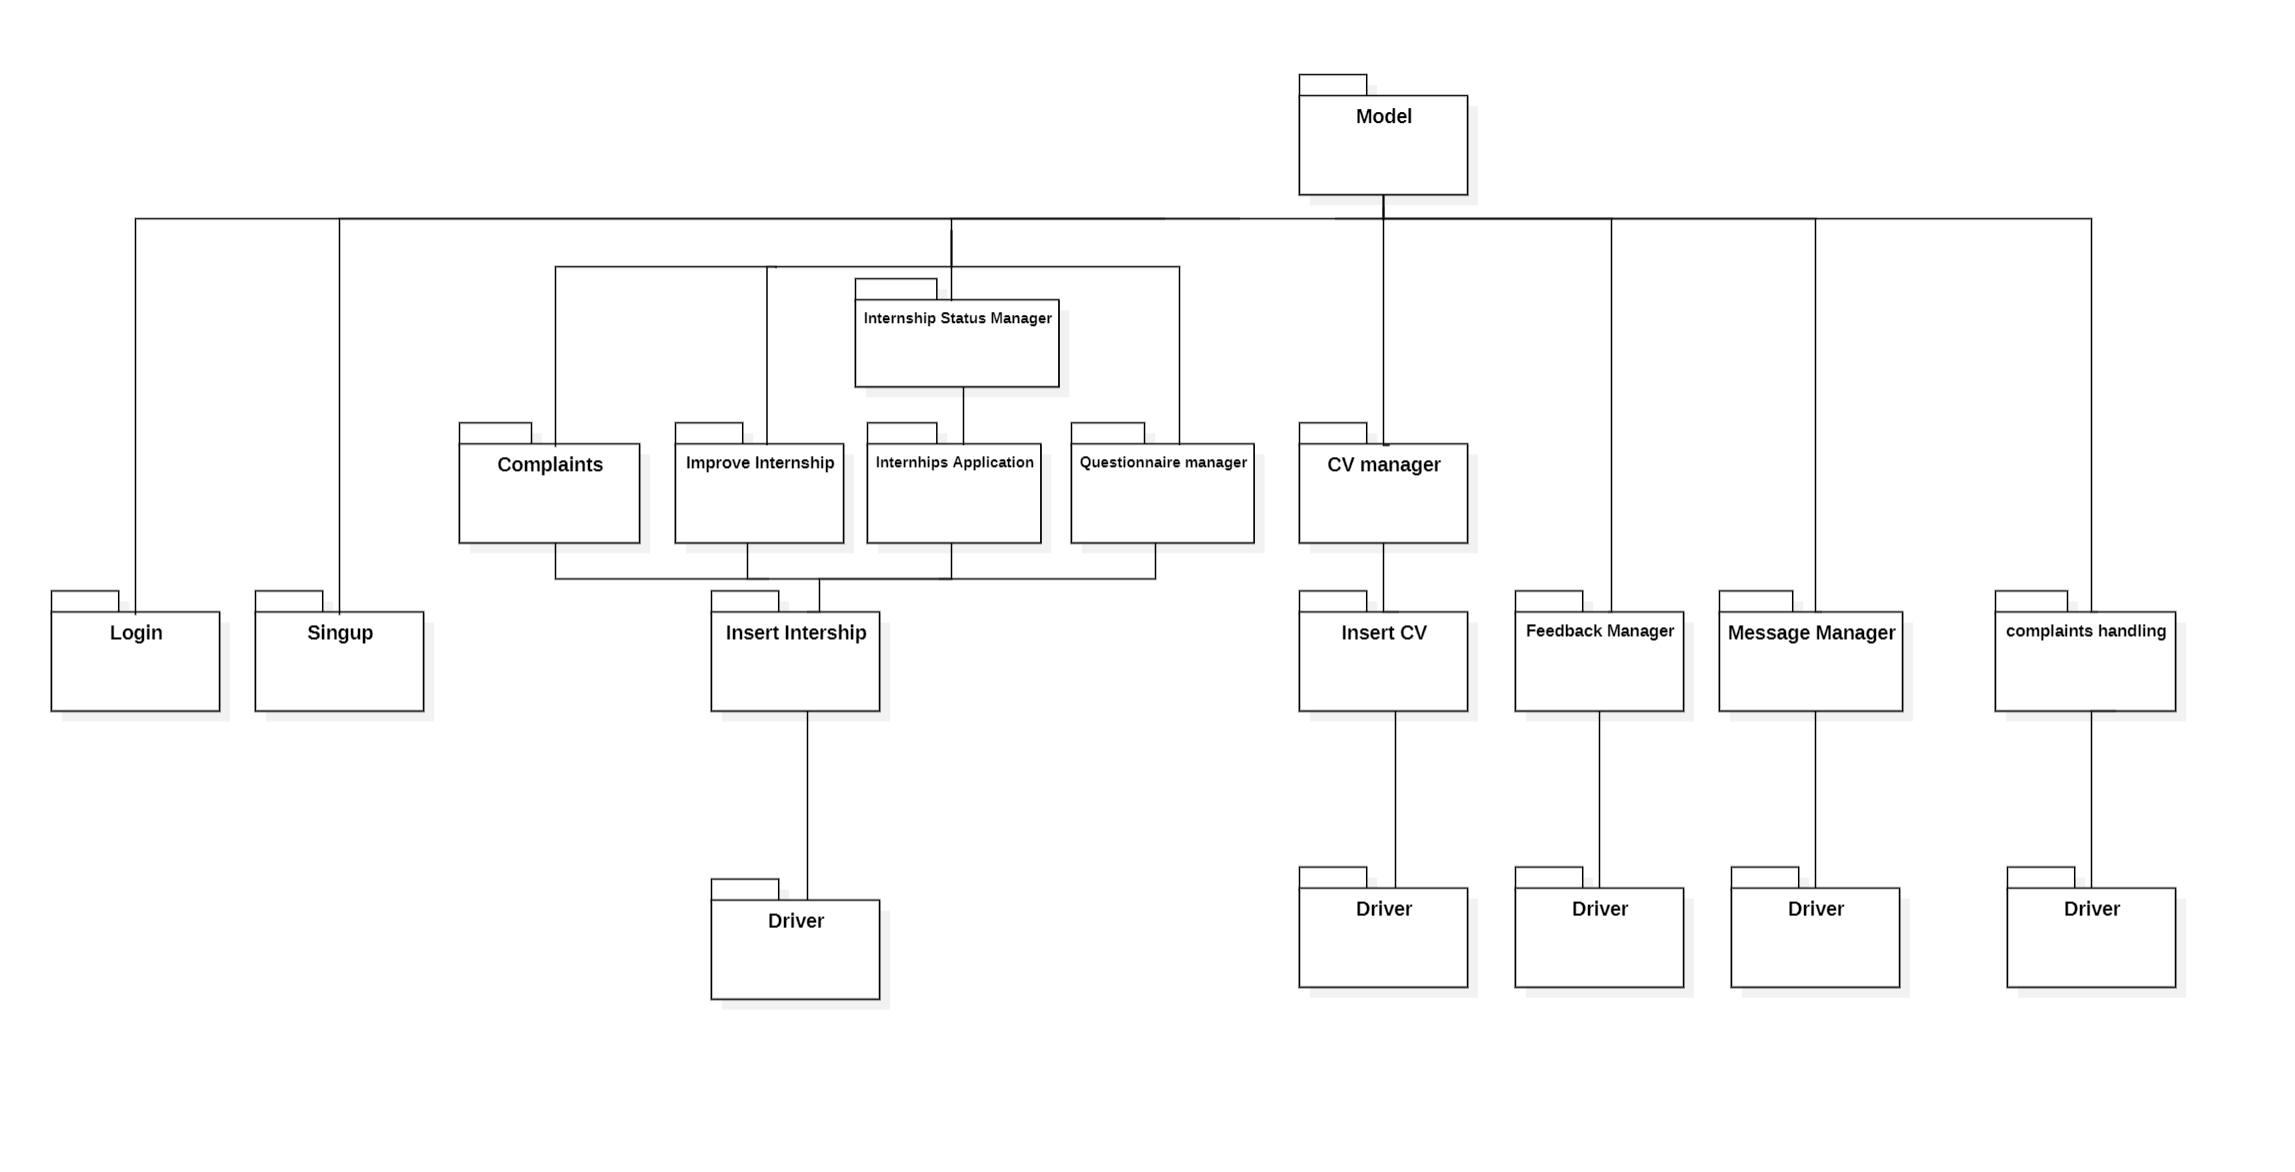
\includegraphics[width=1\linewidth]{DD//Images//Implementation Images/firstmanagers.png}
    \label{fig:enter-label}
\end{figure}

The final component to be integrated is the Dashboard Manager, which is essential for ensuring the proper workflow of the user interface.

\begin{figure}[H]
    \centering
    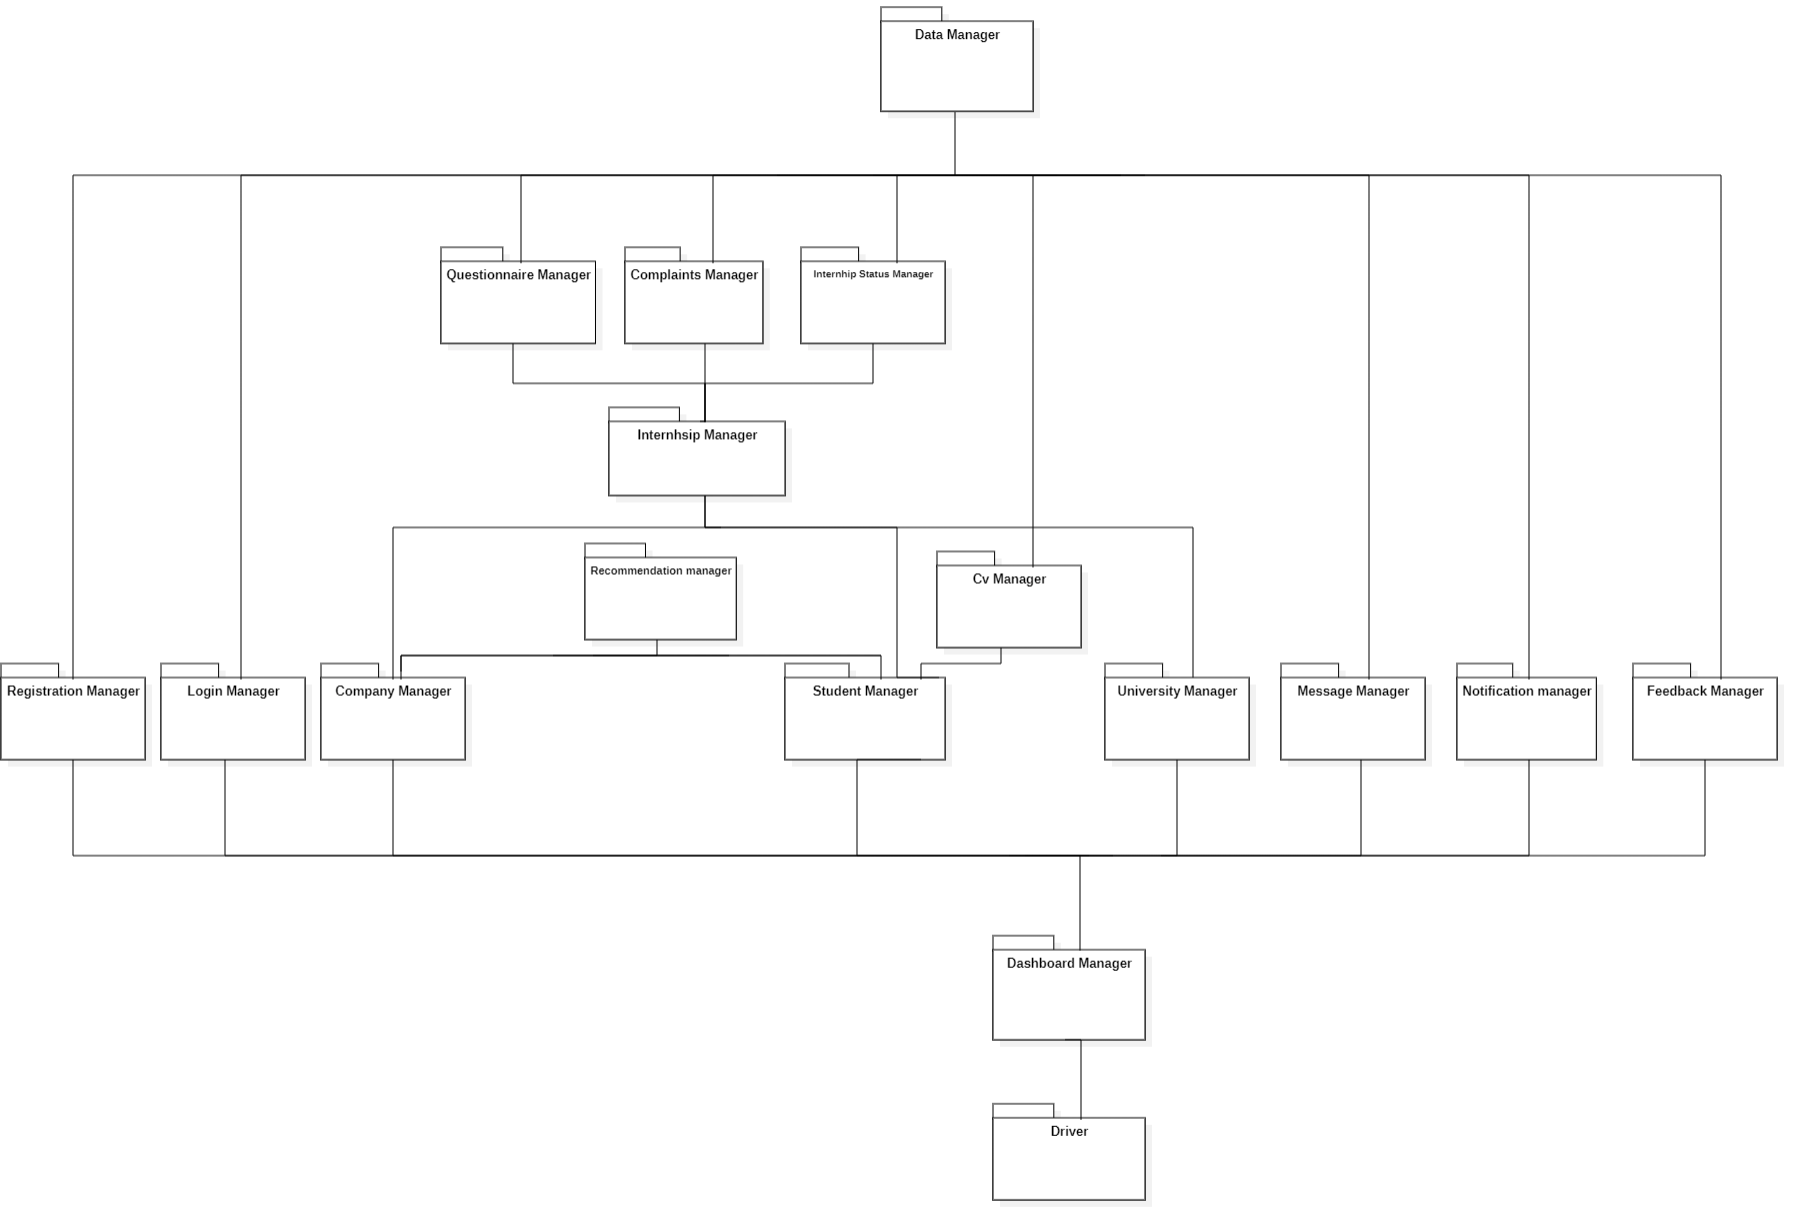
\includegraphics[width=1\linewidth]{DD//Images//Implementation Images/finalmanagers.png}
    \label{fig:enter-label}
\end{figure}

After the removal of the Dashboard Manager's driver, the final system configuration is as follows:

\begin{figure}[H]
    \centering
    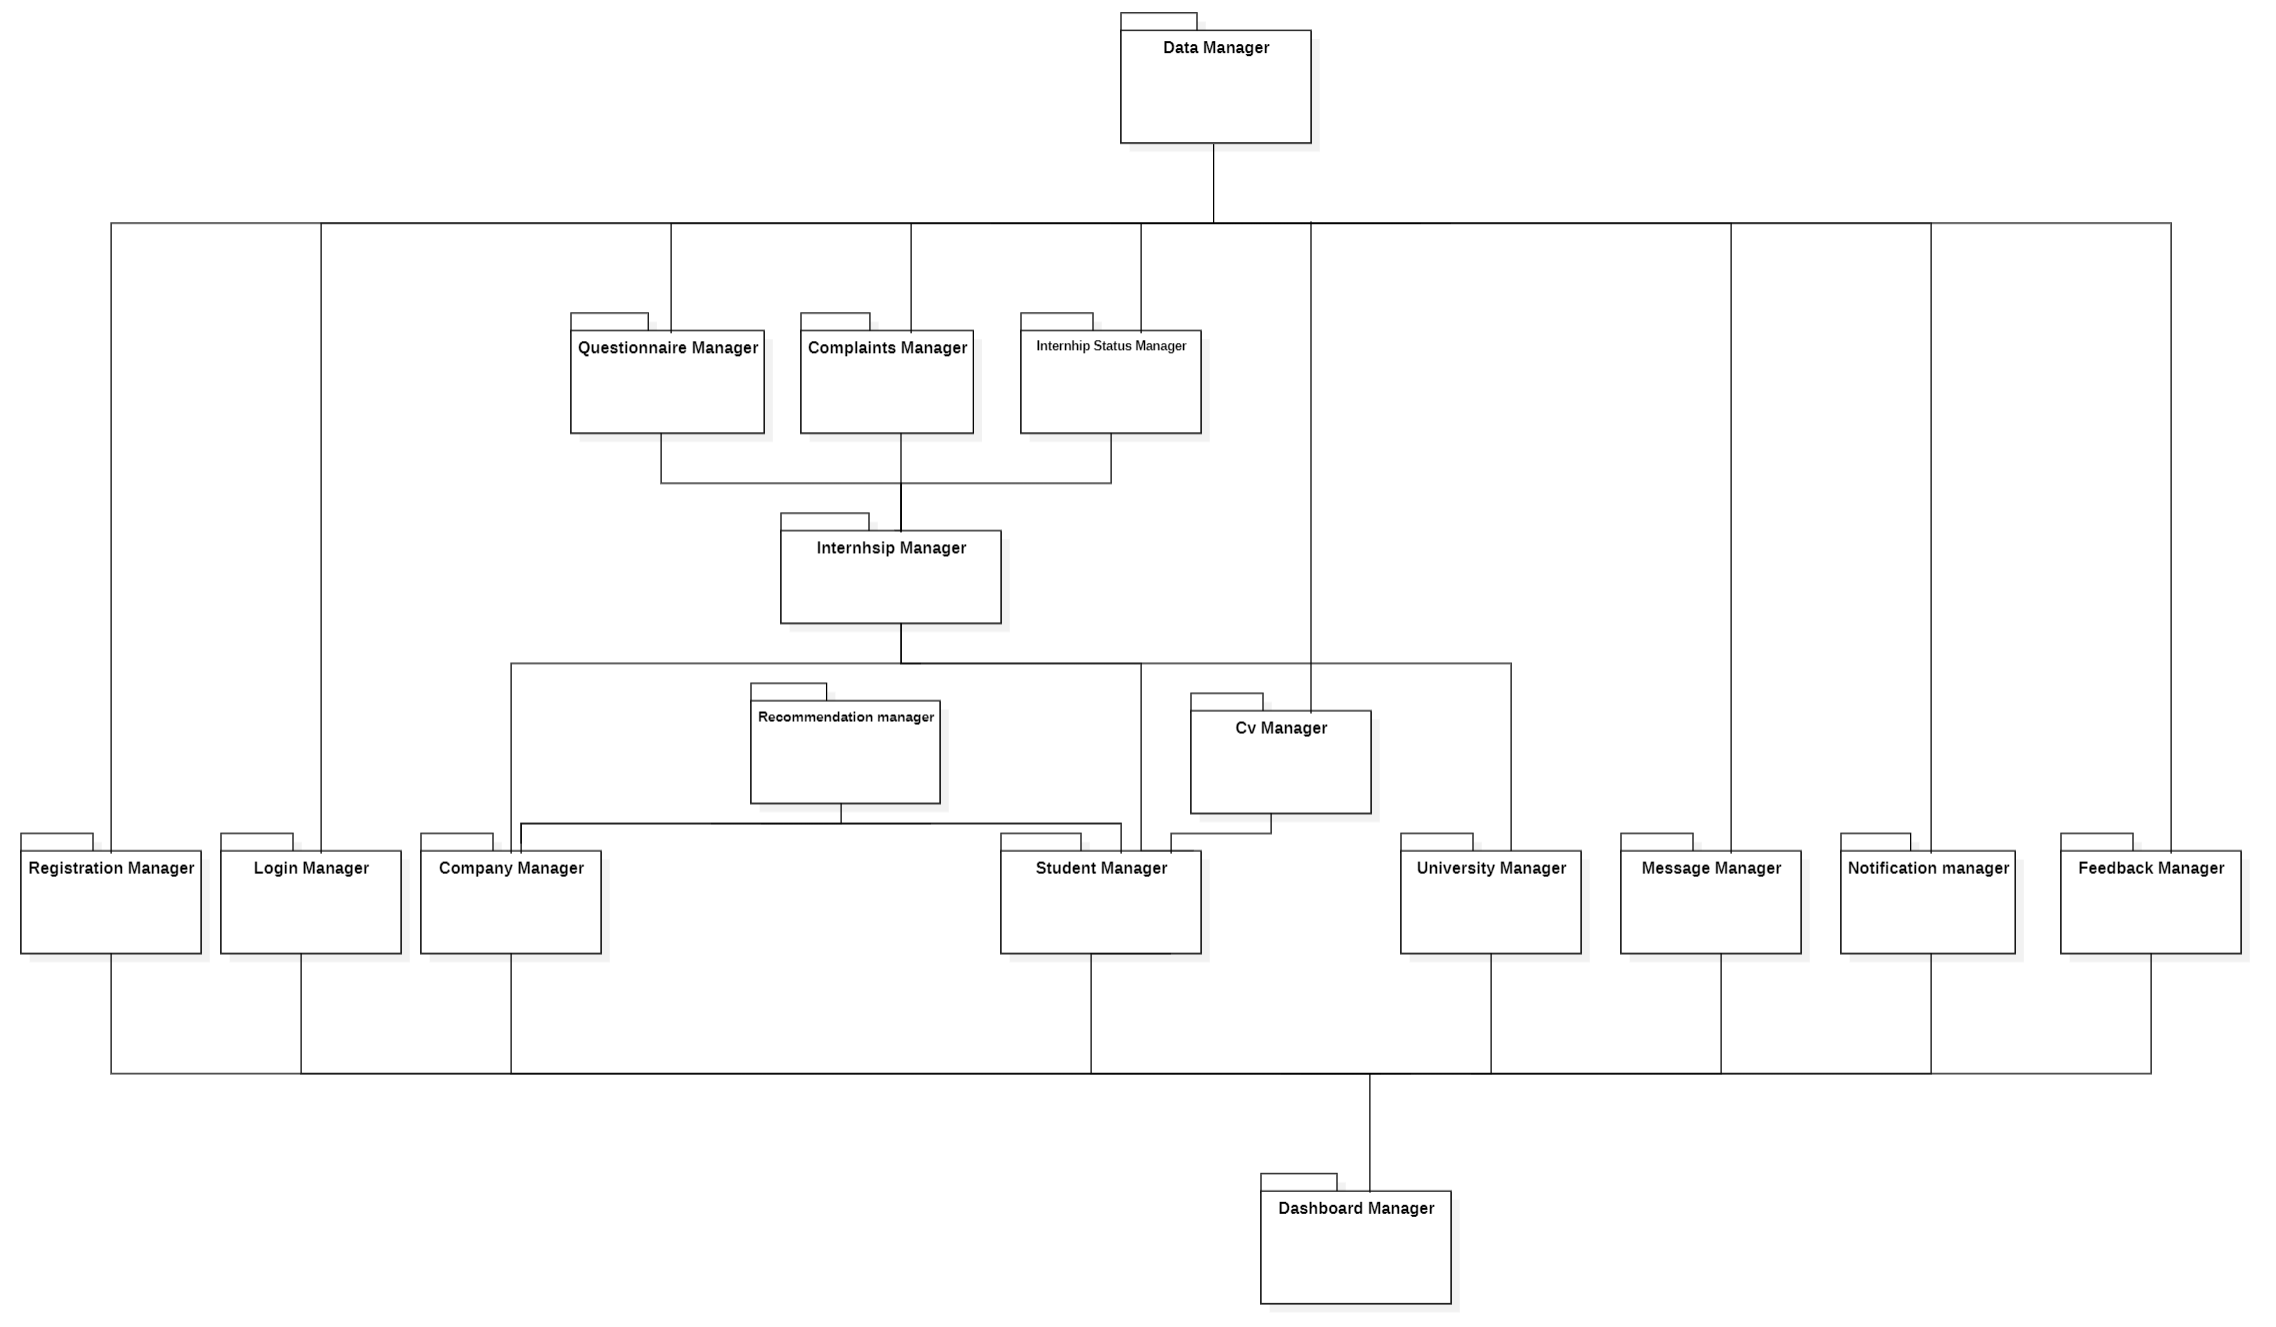
\includegraphics[width=1\linewidth]{DD//Images//Implementation Images/final.png}
    \label{fig:enter-label}
\end{figure}


\section{Integration Strategy}

Thorough testing must be conducted during and after the development phase to ensure that the S\&C performs as expected. The testing aims to validate that the components and overall architecture fulfil the functional and non-functional requirements specified in the RASD document.

\subsection*{Component-Level Testing}
During development, individual components must be tested to validate their functionality. Once a certain component is integrated into the system, it must be checked using stubs and drivers to ensure that the integrated system follows the correct workflow. Once a component passes its individual testing, it is integrated into the larger architecture. After integration, the system is re-tested to ensure functionality and adherence to the workflow.

\subsection*{System-Level Testing}
Once all components are integrated, the system undergoes end-to-end testing. This step verifies the fulfilment of functional and nonfunctional requirements and ensures that the platform operates as intended. The following types of testing are employed:

\begin{itemize}
    \item \textbf{Functional Testing:}  
    This testing verifies that all functional requirements outlined in the RASD document are met. By simulating scenarios described in the use cases, testers ensure the system correctly executes tasks and achieves the expected outcomes.

    \item \textbf{Performance Testing:}  
    Performance testing identifies bottlenecks that could impact response times, utilization, and throughput. It also uncovers inefficiencies in algorithms, hardware, or network configurations. By applying expected workloads and comparing performance metrics, optimization opportunities are identified.

    \item \textbf{Usability Testing:}  
    Usability testing involves observing real users as they interact with the platform. This test ensures that the interface is intuitive, accessible, and user-friendly across various scenarios.

    \item \textbf{Load Testing:}  
    Load testing evaluates the system under increasing workloads to identify its upper operational limits. It helps detect potential issues like memory leaks, buffer overflows, or memory mismanagement. By testing the system for prolonged periods under heavy load, testers ensure stability.

    \item \textbf{Stress Testing:}  
    Stress testing examines the system’s ability to recover from failures. This includes scenarios of resource reduction or overload. The goal is to ensure resilience and fault recovery under extreme conditions.

    \item \textbf{User Interface Testing:}  
    This ensures the system works easily across different devices, browsers, and platforms.
\end{itemize}

\subsection*{Integration and Workflow Validation}
For each newly developed component:

\begin{itemize}
    \item A driver will verify that the component works correctly when integrated into the system.
    \item Subsequent integration tests ensure that existing workflows and module properties remain intact.
\end{itemize}

When all components are fully integrated:

\begin{itemize}
    \item Functional testing will verify workflow consistency, alignment with the RASD document, and fulfillment of specified goals and scenarios.
    \item Load and stress testing will uncover and address memory management issues.
    \item Performance testing will ensure that the system handles simultaneous users efficiently, keeping response times within acceptable limits.
    \item User interface testing will validate usability across devices and platforms.
\end{itemize}

